% FORMATAÇÃO DE TEXTO ==================


\newcommand{\Email}[1]{\href{mailto:#1}{\texttt{#1}}}

\newcommand{\Link}[2][] % Macro para URLs; parâmetro opcional é o texto do hyperlink
  {\href{#2}{\textcolor{CustomTeal}{\ifthenelse{\equal{#1}{}}{\texttt{#2}}{#1}}}}


% COLORAÇÃO DE SINTAXE =================


\newcommand{\SketchPath}[1]{sketches/#1/#1.ino} % Abstração do diretório local de sketches

% Coloração de sintaxe de elementos especiais em código.
\newcommand{\HighlightSpecial}[1]{\textbf{\textcolor{CustomOrange}{#1}}}

% Coloração de sintaxe de valores iniciais de variáveis em código.
\newcommand{\HighlightInit}[1]{\textbf{\textcolor{CustomBrown}{#1}}}

% Coloração de sintaxe de tipos de variáveis em código.
\newcommand{\HighlightType}[1]{\texttt{\textcolor{CustomTeal}{#1}}}


% FRAMES ESPECIAIS =====================


\newcommand{\FinalFrame}{%% Último frame de cada apresentação predefinido
\begin{frame}[focus,b]{Por enquanto é só}\centering
  \begin{columns}[c,onlytextwidth]
  \column{0.7\linewidth}
    Por enquanto é só.
  \column{0.3\linewidth}
    \begin{alertblock}{Material:}
      \medskip
      \href{https://github.com/guilhermgonzaga/MinicursoArduino}%
        {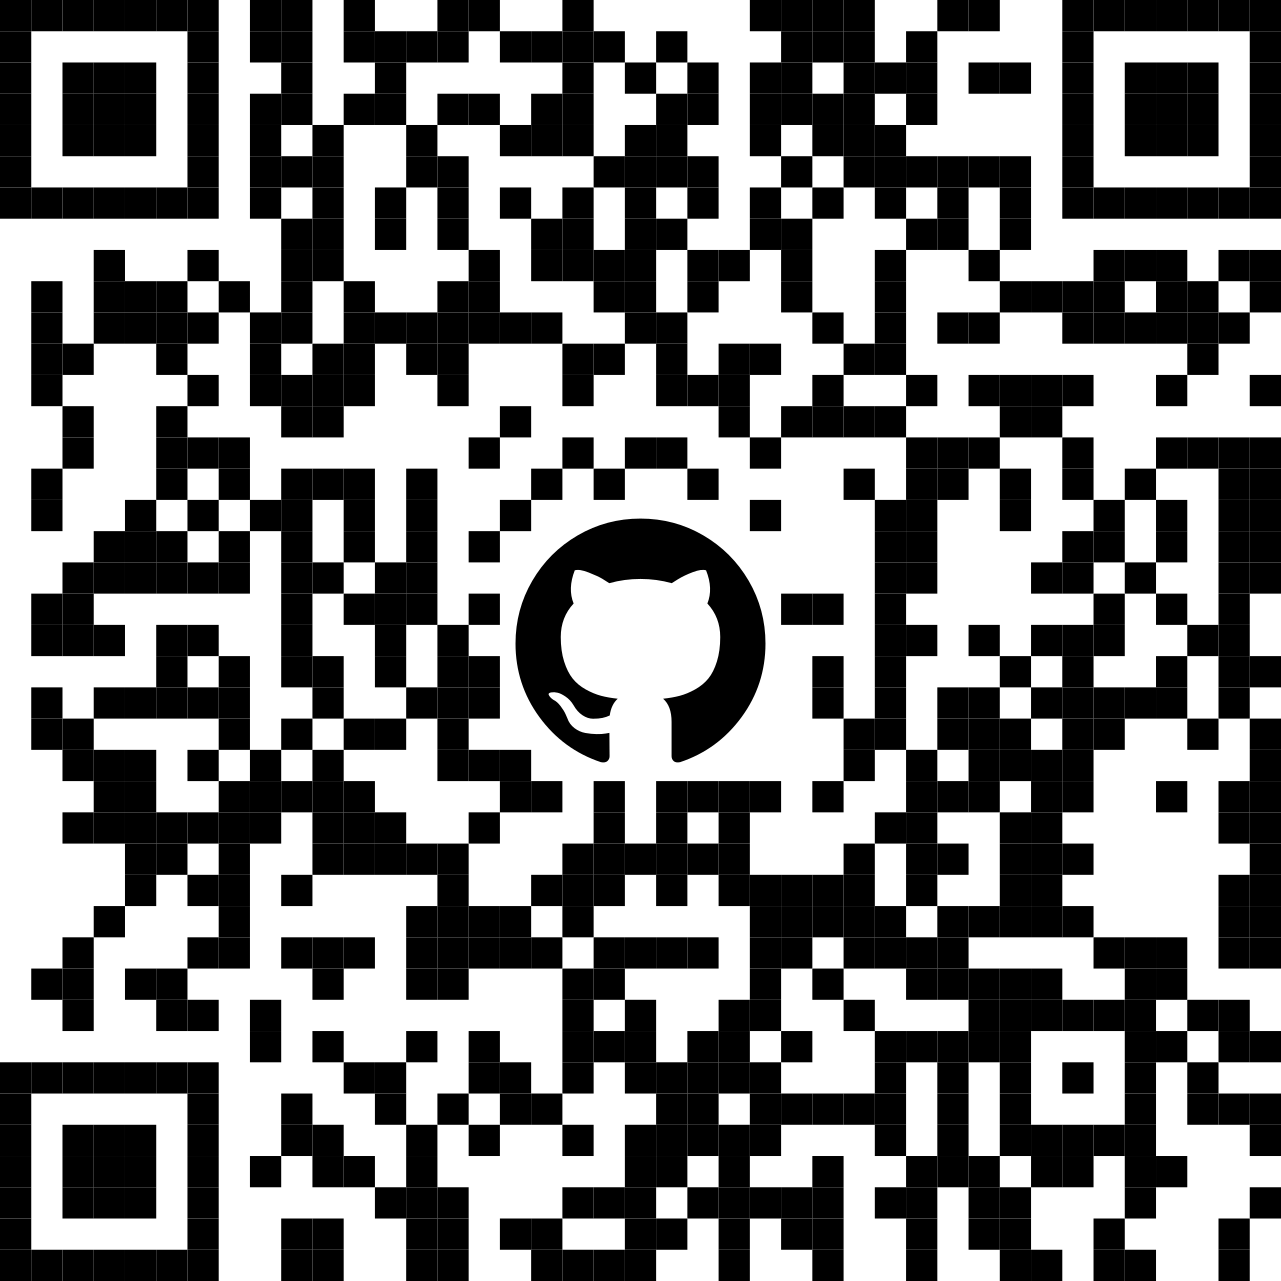
\includegraphics[width=\linewidth]{qrGithub}}
    \end{alertblock}
  \end{columns}
  \vfill
  {\scriptsize \doclicenseThis}
\end{frame}%
}
